\documentclass[12pt,a4paper]{article}
\usepackage{fontspec}
\setmainfont{Times New Roman}
\usepackage{microtype}
\usepackage[a4paper,left=25mm,right=20mm,top=20mm,bottom=18mm,footskip=10mm]{geometry}
\usepackage{graphicx}
\usepackage{tikz}
\usetikzlibrary{positioning,arrows.meta,shapes.geometric,fit,calc}
\usepackage{pdflscape}
\usepackage{fancyhdr}
\usepackage{tabularx}
\usepackage{array}
\usepackage{booktabs}
\usepackage{longtable}
\usepackage{enumitem}
\usepackage{xcolor}
\usepackage{hyperref}
\usepackage{listings}
\usepackage{float}

\definecolor{codegray}{gray}{0.94}
\definecolor{darkgreen}{RGB}{15,62,23}
\hypersetup{colorlinks=true,linkcolor=darkgreen,urlcolor=blue,citecolor=darkgreen}
\setlength{\parindent}{0pt}
\setlength{\parskip}{6pt}
\setlength{\emergencystretch}{3em}
\pagestyle{fancy}
\fancyhf{}
\fancyfoot[C]{\thepage}
\renewcommand{\headrulewidth}{0pt}
\newcommand{\code}[1]{\texttt{\footnotesize\detokenize{#1}}}
\newcommand{\chaptertitle}[1]{\begin{center}{\Large\bfseries #1\par}\end{center}\vspace{8pt}}
\newcommand{\figcaption}[1]{\caption{#1}\label{fig:#1}}
\lstset{basicstyle=\ttfamily\footnotesize,backgroundcolor=\color{codegray},frame=single,breaklines=true}
% Vector diagram source for the FracVision implementation report.
% Included by FracVision_Revised_Project_Report.tex and main.tex.

% Custom Color Palette - Modern, high-contrast, publication-grade
\definecolor{clientbg}{RGB}{240, 246, 255}
\definecolor{clientborder}{RGB}{30, 80, 160}
\definecolor{apibg}{RGB}{236, 243, 255}
\definecolor{apiborder}{RGB}{20, 65, 145}
\definecolor{pipebg}{RGB}{248, 241, 255}
\definecolor{pipeborder}{RGB}{105, 40, 155}
\definecolor{detbg}{RGB}{238, 252, 245}
\definecolor{detborder}{RGB}{25, 125, 75}
\definecolor{clsbg}{RGB}{236, 250, 252}
\definecolor{clsborder}{RGB}{15, 120, 140}
\definecolor{databg}{RGB}{255, 248, 238}
\definecolor{databorder}{RGB}{195, 100, 20}

\tikzset{
  fvbox/.style={draw=black!70, rounded corners=2pt, align=center, minimum height=1.0cm, minimum width=2.8cm, fill=blue!5},
  fvmodel/.style={fvbox, fill=green!10, minimum width=3.1cm},
  fvdata/.style={fvbox, fill=orange!12, minimum width=3.0cm},
  fvext/.style={fvbox, fill=gray!12, minimum width=2.8cm},
  fvdecision/.style={diamond, draw=black!70, align=center, aspect=2, fill=yellow!15, inner sep=2pt},
  fvarrow/.style={->, >=stealth, thick},
  fvline/.style={-, >=stealth, thick},
  % High-visibility architecture styles
  fvbase/.style={draw, line width=1.1pt, rounded corners=5pt, align=center, inner sep=5pt},
  fvclientnode/.style={fvbase, fill=clientbg, draw=clientborder},
  fvapinode/.style={fvbase, fill=apibg, draw=apiborder},
  fvpipenode/.style={fvbase, fill=pipebg, draw=pipeborder},
  fvdetnode/.style={fvbase, fill=detbg, draw=detborder},
  fvclsnode/.style={fvbase, fill=clsbg, draw=clsborder},
  fvdatanode/.style={fvbase, fill=databg, draw=databorder},
  fvarcharrow/.style={-{Latex[length=3mm,width=2.2mm]}, line width=1.2pt, draw=black!75},
  fvbiarrow/.style={{Latex[length=3mm,width=2.2mm]}-{Latex[length=3mm,width=2.2mm]}, line width=1.2pt, draw=black!75},
  fvsubtlelabel/.style={font=\footnotesize\bfseries, fill=white, inner sep=2pt, text=black!85}
}
% Shorthand used inside node text for a readable line break.
\def\n{\\}

\newcommand{\FVOverallArchitecture}{%
\begin{tikzpicture}
  % -------------------------------------------------------------
  % TIER 1: CLIENT & USER INTERFACE LAYER (y = 0)
  % -------------------------------------------------------------
  \node[fvclientnode, text width=6.6cm, minimum height=1.35cm] (user) at (-4.15, 0) {
    {\fontsize{12pt}{14pt}\selectfont\bfseries Clinician / Radiologist}\\[2pt]
    {\fontsize{9.5pt}{12pt}\selectfont Web Browser Client Workstation}
  };

  \node[fvclientnode, text width=8.1cm, minimum height=1.35cm] (frontend) at (3.65, 0) {
    {\fontsize{12pt}{14pt}\selectfont\bfseries Next.js 16 Web Application}\\[2pt]
    {\fontsize{9.5pt}{12pt}\selectfont Interactive Clinical UI · Analyze · Compare · History}
  };

  % -------------------------------------------------------------
  % TIER 2: BACKEND SERVICE & LIFECYCLE CONTROLLER (y = -2.1)
  % -------------------------------------------------------------
  \node[fvapinode, text width=9.8cm, minimum height=1.35cm] (api) at (-2.5, -2.1) {
    {\fontsize{12pt}{14pt}\selectfont\bfseries FastAPI Application Gateway}\\[2pt]
    {\fontsize{9.5pt}{12pt}\selectfont REST API Routes (/predict, /compare, /history) · Validation}
  };

  \node[fvapinode, text width=4.9cm, minimum height=1.35cm] (state) at (5.25, -2.1) {
    {\fontsize{12pt}{14pt}\selectfont\bfseries Pipeline State}\\[2pt]
    {\fontsize{9.5pt}{12pt}\selectfont Lifecycle \& Readiness}
  };

  % -------------------------------------------------------------
  % TIER 3: CORE INFERENCE PIPELINE (y = -4.2)
  % -------------------------------------------------------------
  \node[fvpipenode, text width=15.4cm, minimum height=1.45cm] (pipeline) at (0, -4.2) {
    {\fontsize{12.5pt}{15pt}\selectfont\bfseries FracVision Core Inference Pipeline}\\[3pt]
    {\fontsize{10pt}{13pt}\selectfont Preprocessing (CLAHE, Normalization) $\longrightarrow$ Multi-Model Coordination $\longrightarrow$ Diagnostic Assembly}
  };

  % -------------------------------------------------------------
  % TIER 4: PARALLEL DEEP LEARNING MODEL STREAMS
  % Left Column (x = -3.95): Detection & Segmentation
  % Right Column (x = +3.95): Classification & Progression
  % -------------------------------------------------------------
  \node[fvdetnode, text width=7.3cm, minimum height=1.45cm] (rtdetr) at (-3.95, -6.35) {
    {\fontsize{11.5pt}{14pt}\selectfont\bfseries RT-DETRv2 Detector}\\[2pt]
    {\fontsize{9.5pt}{12pt}\selectfont Real-Time Fracture Detection \& Bounding Boxes}
  };

  \node[fvclsnode, text width=7.3cm, minimum height=1.45cm] (dino) at (3.95, -6.35) {
    {\fontsize{11.5pt}{14pt}\selectfont\bfseries DINOv2 Feature Extractor}\\[2pt]
    {\fontsize{9.5pt}{12pt}\selectfont ViT Foundation Backbone + Classifier Head}
  };

  \node[fvdetnode, text width=7.3cm, minimum height=1.45cm] (seg) at (-3.95, -8.45) {
    {\fontsize{11.5pt}{14pt}\selectfont\bfseries MedSAM Segmentor}\\[2pt]
    {\fontsize{9.5pt}{12pt}\selectfont Prompt-Guided Fracture Mask Segmentation}
  };

  \node[fvclsnode, text width=7.3cm, minimum height=1.45cm] (mamba) at (3.95, -8.45) {
    {\fontsize{11.5pt}{14pt}\selectfont\bfseries Mamba Longitudinal Model}\\[2pt]
    {\fontsize{9.5pt}{12pt}\selectfont Temporal Sequence \& Healing-Stage Prediction}
  };

  % -------------------------------------------------------------
  % TIER 5: PERSISTENCE & BENCHMARK DATASET LAYER (y = -10.65)
  % -------------------------------------------------------------
  \node[fvdatanode, text width=8.8cm, minimum height=1.4cm] (db) at (-3.25, -10.65) {
    {\fontsize{11.5pt}{14pt}\selectfont\bfseries SQLAlchemy Persistence Engine}\\[2pt]
    {\fontsize{9.5pt}{12pt}\selectfont SQLite Default / Production DB · Patients, Studies \& Predictions}
  };

  \node[fvdatanode, text width=5.9cm, minimum height=1.4cm] (datasets) at (4.7, -10.65) {
    {\fontsize{11.5pt}{14pt}\selectfont\bfseries Benchmark Datasets}\\[2pt]
    {\fontsize{9.5pt}{12pt}\selectfont FracAtlas \& GRAZPEDWRI-DX}
  };

  % -------------------------------------------------------------
  % ARROWS & DATA FLOWS (Completely planar, zero crossing!)
  % -------------------------------------------------------------
  % Tier 1: User <-> Frontend
  \draw[fvbiarrow] (user) -- node[above, fvsubtlelabel] {Clinician Actions} (frontend);

  % Tier 1 to Tier 2: Frontend -> API (vertical at x = 1.0)
  \draw[fvbiarrow] (frontend.south -| 1.0, 0) -- node[right, fvsubtlelabel] {HTTPS / REST API} (api.north -| 1.0, 0);

  % Tier 2: API <-> State
  \draw[fvbiarrow] (api) -- node[above, fvsubtlelabel] {Readiness Check} (state);

  % Tier 2 to Tier 3: API -> Pipeline
  \draw[fvarcharrow] (api.south -| pipeline.center) -- node[right, fvsubtlelabel] {Validated Request Tensor} (pipeline.north);

  % Tier 3 to Tier 4: Pipeline to Detection & Classification
  \draw[fvarcharrow] (pipeline.south -| rtdetr.center) -- node[right, fvsubtlelabel] {Input X-ray} (rtdetr.north);
  \draw[fvarcharrow] (pipeline.south -| dino.center) -- node[right, fvsubtlelabel] {Normalized Image} (dino.north);

  % Inside Tier 4: Vertical Intra-Stream Pipelines
  \draw[fvarcharrow] (rtdetr) -- node[right, fvsubtlelabel] {Top Box Prompt} (seg);
  \draw[fvarcharrow] (dino) -- node[right, fvsubtlelabel] {Feature Embeddings} (mamba);

  % Tier 4 to Tier 5: Output Persistence
  \draw[fvarcharrow] (seg) -- node[right, fvsubtlelabel] {Segmentations} (seg |- db.north);
  \draw[fvarcharrow] (mamba) -- node[right, fvsubtlelabel] {Stage Metrics} (mamba |- datasets.north);

  % Datasets to DB
  \draw[fvarcharrow] (datasets) -- (db);
\end{tikzpicture}%
}

\newcommand{\FVWorkflowDiagram}{%
\begin{tikzpicture}[
  x=1cm, y=1cm,
  wfbase/.style={draw, line width=1.2pt, rounded corners=5pt, align=center, inner sep=5pt},
  wfblue/.style={wfbase, fill=blue!8, draw=blue!75!black},
  wfgreen/.style={wfbase, fill=green!10, draw=green!60!black},
  wforange/.style={wfbase, fill=yellow!18, draw=orange!80!black},
  wfpurple/.style={wfbase, fill=purple!8, draw=purple!70!black},
  wfgray/.style={wfbase, fill=gray!12, draw=black!70},
  wfdecision/.style={diamond, draw=orange!80!black, line width=1.2pt, align=center, fill=yellow!20, aspect=2.3, inner sep=2pt, font=\bfseries\normalsize},
  wfarrow/.style={->, >=stealth, line width=1.3pt, draw=black!85},
  lbl/.style={font=\bfseries\small, fill=white, inner sep=1.5pt}
]

  % Tier 1: Ingestion & Validation
  \node[wfgray, text width=6.9cm, minimum height=1.1cm] (upload) at (-4.1, 0) {
    \textbf{\Large 1. Medical Image Upload}\\[2pt]
    \normalsize DICOM, PNG, or JPEG from browser UI
  };
  \node[wfblue, text width=6.9cm, minimum height=1.1cm] (validate) at (4.1, 0) {
    \textbf{\Large 2. FastAPI Validation}\\[2pt]
    \normalsize 50 MB limit \textbullet\ format \& payload check
  };

  % Tier 2: Preprocessing & Quality Control
  \node[wfblue, text width=15.2cm, minimum height=1.1cm] (pre) at (0, -1.65) {
    \textbf{\Large 3. Image Preprocessing \& Quality Control (QC)}\\[2pt]
    \normalsize DICOM decode \textbullet\ Grayscale \textbullet\ CLAHE \textbullet\ Square pad ($1008\times1008$) \textbullet\ Quality check
  };

  % Tier 3: Parallel AI Inference Engines
  % Left Track: Detection & Segmentation
  \node[wfgreen, text width=6.9cm, minimum height=1.1cm] (detect) at (-4.1, -3.35) {
    \textbf{\Large 4a. RT-DETRv2 Detector}\\[2pt]
    \normalsize Fracture bounding boxes ($\ge 0.30$ score)
  };

  \node[wfdecision, text width=2.4cm] (found) at (-4.1, -4.85) {
    Fracture\\Detected?
  };

  \node[wfgreen, text width=6.9cm, minimum height=1.1cm] (segment) at (-4.1, -7.1) {
    \textbf{\Large 4b. MedSAM Segmentation}\\[2pt]
    \normalsize Prompted with primary bbox $\rightarrow$ mask
  };

  % Right Track: Feature Extraction & Classification
  \node[wfpurple, text width=6.9cm, minimum height=1.1cm] (dino) at (4.1, -3.35) {
    \textbf{\Large 5a. DINOv2 ViT Extractor}\\[2pt]
    \normalsize ViT-S/14 encoder $\rightarrow$ feature representation
  };

  \node[wfpurple, text width=6.9cm, minimum height=1.1cm] (classify) at (4.1, -7.1) {
    \textbf{\Large 5b. Multilabel Classifier}\\[2pt]
    \normalsize Linear / MLP head \textbullet\ Class probabilities
  };

  % Tier 4: Unified Prediction Assembly
  \node[wfblue, text width=15.2cm, minimum height=1.1cm] (result) at (0, -8.95) {
    \textbf{\Large 6. Unified Prediction Result Assembly}\\[2pt]
    \normalsize Aggregates QC status, bounding boxes, masks, probabilities, and stage errors
  };

  % Tier 5: Persistence & UI
  \node[wforange, text width=6.9cm, minimum height=1.1cm] (persist) at (-4.1, -10.7) {
    \textbf{\Large 7a. Database Persistence}\\[2pt]
    \normalsize SQLite DB \textbullet\ Patient \& prediction JSON
  };
  \node[wfpurple, text width=6.9cm, minimum height=1.1cm] (ui) at (4.1, -10.7) {
    \textbf{\Large 7b. Interactive Web UI}\\[2pt]
    \normalsize Next.js UI \textbullet\ Canvas overlay \& mask
  };

  % Connectors
  % 1 -> 2
  \draw[wfarrow] (upload) -- (validate);
  % 2 -> 3
  \draw[wfarrow] (validate.south) -- (validate.south |- pre.north);

  % 3 -> 4a (left track) and 3 -> 5a (right track)
  \draw[wfarrow] (pre.south -| detect.north) -- (detect.north);
  \draw[wfarrow] (pre.south -| dino.north) -- (dino.north);

  % Left track: 4a -> found -> 4b (Yes)
  \draw[wfarrow] (detect) -- (found);
  \draw[wfarrow] (found) -- node[lbl, text=green!60!black, left=2pt]{Yes} (segment);
  
  % Left track: found -> No (skip mask) -> result
  \draw[wfarrow] (found.east) -- ++(1.8, 0) node[above, font=\bfseries\small, text=red!75!black, midway]{No (skip mask)} |- ([xshift=-1.5cm]result.north);

  % Left track: 4b -> result
  \draw[wfarrow] (segment.south) -- (segment.south |- result.north);

  % Right track: 5a -> 5b (with embedding label) -> result
  \draw[wfarrow] (dino) -- node[lbl, text=black!75]{384-D CLS embedding} (classify);
  \draw[wfarrow] (classify.south) -- (classify.south |- result.north);

  % Result -> 7a (Database) and 7b (UI)
  \draw[wfarrow] (result.south -| persist.north) -- (persist.north);
  \draw[wfarrow] (result.south -| ui.north) -- (ui.north);

\end{tikzpicture}%
}

\newcommand{\FVModelPipeline}{%
\begin{tikzpicture}[node distance=0.65cm and 0.75cm, font=\small]
  \node[fvdata] (img) {Input X-ray\\H×W×1/3};
  \node[fvbox, right=of img] (norm) {Square padded tensor\\1008×1008 configured\\mean/std normalization};
  \node[fvmodel, right=of norm] (rtdetr) {RT-DETRv2\\classes from config\\boxes + scores + labels};
  \node[fvmodel, right=of rtdetr] (medsam) {MedSAM\\fracture bbox prompt\\mask + score + area};
  \node[fvmodel, below=of rtdetr] (dino) {DINOv2 ViT-S/14\\384-D CLS token\\patch tokens available};
  \node[fvmodel, right=of dino] (clf) {FractureClassifier\\linear/MLP head\\FocalLoss α=.25 γ=2};
  \node[fvbox, below=of clf] (cal) {Optional temperature\\scaling calibration};
  \node[fvbox, below=of medsam] (out) {PredictionResult\\partial results preserved\\stage\_errors per stage};
  \draw[fvarrow] (img) -- (norm);
  \draw[fvarrow] (norm) -- (rtdetr);
  \draw[fvarrow] (rtdetr) -- (medsam);
  \draw[fvarrow] (norm) |- (dino);
  \draw[fvarrow] (dino) -- (clf);
  \draw[fvarrow] (clf) -- (cal);
  \draw[fvarrow] (medsam) -- (out);
  \draw[fvarrow] (cal) -- (out);
\end{tikzpicture}%
}

\newcommand{\FVDataFlowDiagram}{%
\begin{tikzpicture}[
  actor/.style={draw=black!70, fill=gray!12, rounded corners=5pt, line width=1.1pt, align=center, inner sep=5pt, text width=4.0cm, minimum height=1.2cm},
  front/.style={draw=blue!75!black, fill=blue!8, rounded corners=5pt, line width=1.1pt, align=center, inner sep=5pt, text width=7.8cm, minimum height=1.2cm},
  api/.style={draw=blue!85!black, fill=blue!12, rounded corners=5pt, line width=1.2pt, align=center, inner sep=6pt, text width=15.4cm, minimum height=1.4cm},
  tempbox/.style={draw=orange!80!black, fill=yellow!18, dashed, rounded corners=5pt, line width=1.1pt, align=center, inner sep=5pt, text width=5.6cm, minimum height=1.4cm},
  pipebox/.style={draw=purple!70!black, fill=purple!8, rounded corners=5pt, line width=1.1pt, align=center, inner sep=5pt, text width=7.4cm, minimum height=1.4cm},
  dbbox/.style={draw=orange!80!black, fill=orange!12, rounded corners=5pt, line width=1.1pt, align=center, inner sep=5pt, text width=5.6cm, minimum height=1.6cm},
  jsonbox/.style={draw=green!65!black, fill=green!12, rounded corners=5pt, line width=1.2pt, align=center, inner sep=5pt, text width=7.4cm, minimum height=1.6cm},
  arrow/.style={->, >=stealth, line width=1.2pt, draw=black!85},
  darrow/.style={<->, >=stealth, line width=1.2pt, draw=black!85},
  lbl/.style={font=\fontsize{9pt}{11pt}\selectfont\bfseries, fill=white, inner sep=2pt, text=black!90}
]

  % Row 1: Presentation Layer (y = 0)
  \node[actor] (user) at (-5.7, 0) {
    {\fontsize{11.5pt}{14pt}\selectfont\bfseries User / Clinician}\\[2pt]
    {\fontsize{9pt}{11.5pt}\selectfont Browser Interface}
  };
  \node[front] (ui) at (3.8, 0) {
    {\fontsize{11.5pt}{14pt}\selectfont\bfseries Next.js Web Frontend}\\[2pt]
    {\fontsize{9pt}{11.5pt}\selectfont Upload Page \;\textbullet\; Serial Compare \;\textbullet\; History View}
  };

  % Row 2: API Gateway Layer (y = -2.2)
  \node[api] (api) at (0, -2.2) {
    {\fontsize{12pt}{14.5pt}\selectfont\bfseries FastAPI Backend Gateway}\\[3pt]
    {\fontsize{9pt}{11.5pt}\selectfont Input validation \;\textbullet\; Pydantic models \;\textbullet\; Temporary file management}\\[2pt]
    {\fontsize{9pt}{11.5pt}\selectfont Endpoints: \texttt{POST /api/predict} (multipart) \;\textbullet\; \texttt{GET /api/history} (JSON)}
  };

  % Row 3: Processing & Buffering Layer (y = -4.8)
  \node[tempbox] (temp) at (-5.1, -4.8) {
    {\fontsize{11pt}{13.5pt}\selectfont\bfseries Temporary File Buffer}\\[2pt]
    {\fontsize{9pt}{11.5pt}\selectfont \texttt{/tmp/upload\_*.ext} (DICOM decode)}\\[2pt]
    {\fontsize{8.5pt}{10.5pt}\selectfont\itshape Written for decode, auto-deleted}
  };
  \node[pipebox] (pipe) at (4.1, -4.8) {
    {\fontsize{11.5pt}{14pt}\selectfont\bfseries Multi-Stage Pipeline}\\[2pt]
    {\fontsize{9pt}{11.5pt}\selectfont NumPy tensors $\longrightarrow$ RT-DETR $\longrightarrow$ MedSAM}\\[2pt]
    {\fontsize{8.5pt}{11pt}\selectfont QC $\longrightarrow$ Detection $\longrightarrow$ Segmentation $\longrightarrow$ Classification}
  };

  % Row 4: Persistence & Output Serialization (y = -7.9)
  \node[dbbox] (db) at (-5.1, -7.9) {
    {\fontsize{11.5pt}{14pt}\selectfont\bfseries SQLAlchemy Database}\\[2pt]
    {\fontsize{9pt}{11.5pt}\selectfont SQLite default / configured DB}\\[2pt]
    {\fontsize{8.5pt}{11pt}\selectfont Patients, Studies \& Predictions}\\[2pt]
    {\fontsize{8.5pt}{10.5pt}\selectfont\itshape Queried for historical reviews}
  };
  \node[jsonbox] (json) at (4.1, -7.9) {
    {\fontsize{11.5pt}{14pt}\selectfont\bfseries Prediction JSON \& Overlays}\\[2pt]
    {\fontsize{9pt}{11.5pt}\selectfont Bounding boxes \;\textbullet\; Probabilities \;\textbullet\; Mask URL}\\[2pt]
    {\fontsize{8.5pt}{11pt}\selectfont Canvas overlay rendering \;\textbullet\; Clinical disclaimer}\\[2pt]
    {\fontsize{8.5pt}{10.5pt}\selectfont\bfseries validated = false \textnormal{research flag}}
  };

  % Connectors
  % Row 1
  \draw[arrow] (user) -- node[lbl, above=3pt]{Upload / Review} (ui);

  % Row 1 to Row 2
  \draw[darrow] (ui.south -| 3.8, 0) -- node[lbl, right=5pt]{HTTP Requests / Responses} (api.north -| 3.8, 0);

  % Row 2 to Row 3
  \draw[arrow] (api.south -| temp.north) -- node[lbl, left=5pt]{Write / Delete} (temp.north);
  \draw[arrow] (api.south -| pipe.north) -- node[lbl, right=5pt]{Execute Tensors} (pipe.north);

  % Row 3 to Row 4 (Multi-stage -> Prediction JSON)
  \draw[arrow] (pipe) -- node[lbl, right=5pt]{Generate Results} (json);

  % Row 4 Horizontal: Persist JSON
  \draw[arrow] (json.west) -- node[lbl, above=3pt]{Persist JSON} (db.east);

  % Database to API: History Query
  \draw[arrow] (db.west) -- ++(-1.0, 0) |- node[lbl, pos=0.45, left=5pt]{History Query} (api.west);

\end{tikzpicture}%
}

\newcommand{\FVDatabaseDiagram}{%
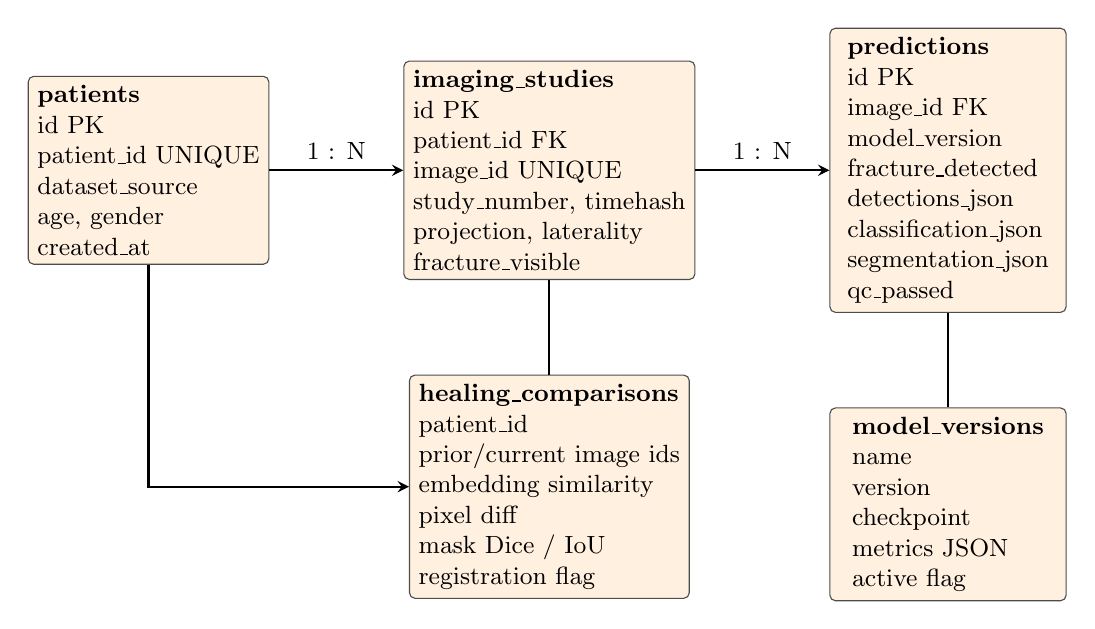
\begin{tikzpicture}[node distance=1.2cm and 1.7cm, font=\small]
  \node[fvdata, align=left] (patient) {\textbf{patients}\\id PK\\patient\_id UNIQUE\\dataset\_source\\age, gender\\created\_at};
  \node[fvdata, right=of patient, align=left] (study) {\textbf{imaging\_studies}\\id PK\\patient\_id FK\\image\_id UNIQUE\\study\_number, timehash\\projection, laterality\\fracture\_visible};
  \node[fvdata, right=of study, align=left] (pred) {\textbf{predictions}\\id PK\\image\_id FK\\model\_version\\fracture\_detected\\detections\_json\\classification\_json\\segmentation\_json\\qc\_passed};
  \node[fvdata, below=of study, align=left] (comp) {\textbf{healing\_comparisons}\\patient\_id\\prior/current image ids\\embedding similarity\\pixel diff\\mask Dice / IoU\\registration flag};
  \node[fvdata, below=of pred, align=left] (version) {\textbf{model\_versions}\\name\\version\\checkpoint\\metrics JSON\\active flag};
  \draw[fvarrow] (patient) -- node[above]{1 : N} (study);
  \draw[fvarrow] (study) -- node[above]{1 : N} (pred);
  \draw[fvarrow] (patient) |- (comp);
  \draw[fvline] (study) -- (comp);
  \draw[fvline] (version) -- (pred);
\end{tikzpicture}%
}

\newcommand{\FVValidationDiagram}{%
\begin{tikzpicture}[
  font=\large,
  vbox/.style={draw=blue!75!black, fill=blue!8, rounded corners=6pt, line width=1.3pt, align=center, inner sep=6pt, text width=8.6cm},
  vdec/.style={draw=orange!90!black, fill=yellow!18, rounded corners=6pt, line width=1.3pt, align=center, inner sep=6pt, text width=7.4cm, font=\large\bfseries},
  verr/.style={draw=red!75!black, fill=red!10, rounded corners=5pt, line width=1.2pt, align=center, inner sep=6pt, text width=5.8cm, font=\normalsize},
  vwarn/.style={draw=orange!85!black, fill=orange!12, rounded corners=5pt, line width=1.2pt, align=center, inner sep=6pt, text width=5.8cm, font=\normalsize},
  vresp/.style={draw=green!65!black, fill=green!12, rounded corners=6pt, line width=1.4pt, align=center, inner sep=7pt, text width=8.6cm},
  varrow/.style={->, >=stealth, line width=1.4pt, draw=black!85},
  tagyes/.style={font=\large\bfseries, fill=white, text=green!60!black, inner sep=2pt},
  tagno/.style={font=\large\bfseries, fill=white, text=red!75!black, inner sep=2pt}
]

  % 1. Incoming Request
  \node[vbox] (req) {\textbf{\Large Client Request}\\\normalsize Upload X-ray Image (DICOM, PNG, or JPEG)};
  
  % 2. Gate 1: Pipeline Readiness
  \node[vdec, below=0.55cm of req] (ready) {Is Pipeline Ready?\\\normalsize\normalfont Checkpoint \& service initialized};
  \node[verr, right=1.0cm of ready] (err503) {\textbf{\large HTTP 503 Load Error}\\Model checkpoints or pipeline state missing};
  
  % 3. Gate 2: File Validation
  \node[vdec, below=0.55cm of ready] (valid) {Valid Size \& Format?\\\normalsize\normalfont File size $\le$ 50 MB, valid suffix};
  \node[verr, right=1.0cm of valid] (err413) {\textbf{\large HTTP 413 / 415 Error}\\File oversized or unsupported format};
  
  % 4. Multi-Stage Pipeline Execution
  \node[vbox, below=0.55cm of valid, text width=8.6cm] (exec) {\textbf{\Large Execute Pipeline Stages (try / except)}\\\normalsize Preprocess $\rightarrow$ Detect $\rightarrow$ Segment $\rightarrow$ Classify};
  
  % 5. Fault Isolation: Stage Error Check
  \node[vdec, below=0.55cm of exec] (stage) {Any Stage-Level Error?\\\normalsize\normalfont Exception caught during stage};
  \node[vwarn, right=1.0cm of stage] (errstage) {\textbf{\large Degraded Mode Execution}\\Record stage failure; continue remaining stages};
  
  % 6. Structured Safe Response
  \node[vresp, below=0.55cm of stage] (resp) {\textbf{\Large HTTP 200 Success Response}\\\large\textbf{validated = false} \;\textbullet\; Non-Clinical Disclaimer\\\normalsize Prediction JSON + Mask URL + Heatmaps + Status Flags};

  % Connectors
  \draw[varrow] (req) -- (ready);
  
  \draw[varrow] (ready) -- node[tagno, above]{No} (err503);
  \draw[varrow] (ready) -- node[tagyes, right]{Yes} (valid);
  
  \draw[varrow] (valid) -- node[tagno, above]{No} (err413);
  \draw[varrow] (valid) -- node[tagyes, right]{Yes} (exec);
  
  \draw[varrow] (exec) -- (stage);
  
  \draw[varrow] (stage) -- node[tagno, above]{Yes} (errstage);
  \draw[varrow] (stage) -- node[tagyes, right]{No} (resp);
  
  \draw[varrow] (errstage) |- (resp);

\end{tikzpicture}%
}


\begin{document}

\begin{titlepage}
\thispagestyle{empty}
\begin{center}
{\Large\bfseries VALIA KOONAMBAIKULATHAMMA COLLEGE OF ENGINEERING \& TECHNOLOGY\par}
\vspace{8pt}
{\large\bfseries DEPARTMENT OF COMPUTER SCIENCE AND ENGINEERING\par}
\vspace{25pt}
{\Large\bfseries FRACVISION\par}
\vspace{7pt}
{\large\bfseries Multimodal X-ray Fracture Analysis and Longitudinal\par}
{\large\bfseries Healing-Stage Research Prototype\par}
\vspace{20pt}
{\large PROJECT REPORT\par}
\vspace{12pt}
Submitted by
\vspace{8pt}
\begin{tabular}{c}
\textbf{Adwaith S} \quad VKE23CS006\\
\textbf{Aswathy P} \quad VKE23CS019\\
\textbf{Sohan Antony} \quad VKE23CS045\\
\textbf{Sreenandha M} \quad VKE23CS046
\end{tabular}
\vfill
\textbf{Project Guide:} Reeba B\\
\textbf{Project Coordinator:} Dr Shine Raj G\\
\textbf{Head of the Department:} Dr. Shine Raj G
\vspace{18pt}

SEPTEMBER 2026
\end{center}
\end{titlepage}

\pagenumbering{roman}
\section*{DECLARATION}
We, \textbf{Adwaith S, Aswathy P, Sohan Antony, and Sreenandha M}, declare that this project report entitled \textbf{“FracVision: Multimodal X-ray Fracture Analysis and Longitudinal Healing-Stage Research Prototype”} is our original work carried out under the guidance of Reeba B. The report describes the implementation present in the supplied FracVision repository. It does not claim clinical validation, autonomous diagnosis, or trained performance results that are not supported by the repository artifacts.

\vspace{18pt}
\hfill Adwaith S\\
\hfill Aswathy P\\
\hfill Sohan Antony\\
\hfill Sreenandha M

\newpage
\section*{CERTIFICATE}
This is to certify that the project report entitled \textbf{“FracVision: Multimodal X-ray Fracture Analysis and Longitudinal Healing-Stage Research Prototype”} submitted by \textbf{Adwaith S [VKE23CS006], Aswathy P [VKE23CS019], Sohan Antony [VKE23CS045], and Sreenandha M [VKE23CS046]} is a bonafide record of the project work carried out under the guidance of Reeba B.

\vspace{25pt}
\begin{tabularx}{\textwidth}{XXX}
\textbf{Project Guide} & \textbf{Project Coordinator} & \textbf{Head of the Department}\\[8pt]
Reeba B & Dr Shine Raj G & Dr. Shine Raj G\\
Assistant Professor & Assistant Professor & Professor\\
Department of CSE & Department of CSE & Department of CSE\\
VKCET & VKCET & VKCET
\end{tabularx}

\newpage
\section*{ACKNOWLEDGEMENT}
We express our sincere gratitude to our project guide, \textbf{Reeba B}, for her guidance and technical supervision. We thank \textbf{Dr Shine Raj G}, Project Coordinator, for his coordination and support, and \textbf{Dr. Shine Raj G}, Head of the Department of Computer Science and Engineering, for providing the academic environment and facilities required for the project. We also thank the faculty members and staff of VKCET for their assistance throughout the project.

\vspace{18pt}
\hfill \textbf{Adwaith S, Aswathy P, Sohan Antony, Sreenandha M}

\newpage
\section*{ABSTRACT}
FracVision is a modular research prototype for multimodal analysis of bone X-ray images. The implementation combines image quality control and preprocessing with four model-oriented components: RT-DETRv2 for fracture-related object detection, MedSAM for box-prompted segmentation, DINOv2 for visual feature extraction, and a configurable multilabel classifier operating on DINOv2 embeddings. A Mamba-style longitudinal model is also implemented for sequence-level healing-stage classification when serial patient studies and appropriate labels are available. The application is exposed through a FastAPI service and a Next.js web interface that supports single-image analysis, serial comparison, and prediction history.

The verified codebase is intentionally conservative about medical claims. Every prediction carries a non-clinical disclaimer, outputs include quality-control status and stage-level errors, and supervised recovery-time training is disabled because the configured datasets do not provide verified time-to-union or censoring labels. The repository contains model interfaces, adapters, training scripts, evaluation utilities, tests, and deployment configuration, but the supplied snapshot contains no dataset files or trained checkpoint artifacts. Accordingly, this report documents the implemented architecture and algorithms without fabricating accuracy, latency, or clinical performance values.

\newpage
\tableofcontents
\newpage
\listoffigures
\newpage
\listoftables
\newpage
\section*{LIST OF SYMBOLS AND ABBREVIATIONS}
\begin{tabularx}{\textwidth}{>{\bfseries}lX}
AI & Artificial Intelligence\\
API & Application Programming Interface\\
CLAHE & Contrast Limited Adaptive Histogram Equalization\\
DICOM & Digital Imaging and Communications in Medicine\\
IoU & Intersection over Union\\
QC & Quality Control\\
SSM & State Space Model\\
VOC & Pascal Visual Object Classes\\
YOLO & You Only Look Once annotation format
\end{tabularx}

\clearpage
\pagenumbering{arabic}
\section{Introduction}
\subsection{Background and project overview}
Radiographic fracture analysis requires more than a binary image label. A usable analysis workflow may need to check input quality, localize suspicious regions, create a pixel-level region estimate, classify image-level attributes, and compare serial studies. FracVision implements these concerns as a modular research system rather than as one monolithic predictor.

The repository identifies the system as \textbf{FracVision}, version 0.1.0. Its primary application path is a browser-based Next.js interface communicating with a FastAPI backend. The backend loads an inference pipeline during the application lifespan and maps model outputs into typed Pydantic responses. A SQLAlchemy persistence layer stores de-identified prediction history. The model package contains adapters for FracAtlas and GRAZPEDWRI-DX, preprocessing, pairing, training, inference, and evaluation utilities.

\subsection{Problem statement}
The problem addressed is the engineering of a reproducible, multimodal X-ray analysis workflow that can expose detection, segmentation, classification, and serial-comparison outputs through one application interface while preserving uncertainty and safety information. The implementation does not solve autonomous clinical diagnosis. It provides a research and integration foundation in which each stage can fail independently and report its status.

\subsection{Objectives}
\begin{enumerate}[leftmargin=*]
\item Standardize JPEG, PNG, and DICOM inputs through configurable quality-control preprocessing.
\item Detect fracture-related regions and return pixel-coordinate bounding boxes with confidence scores.
\item Use the highest-confidence fracture box as an optional MedSAM prompt for segmentation.
\item Extract DINOv2 visual features and produce multilabel probabilities through a classifier head.
\item Compare serial images using registration, embedding similarity, pixel differences, and mask overlap.
\item Provide longitudinal sequence modelling with a Mamba-style model while disabling unsupported recovery-time supervision.
\item Serve results through typed REST endpoints and present overlays, probabilities, warnings, and history in a web UI.
\end{enumerate}

\subsection{Scope and boundaries}
The scope includes the implemented software, model interfaces, data adapters, configuration, API, frontend, persistence, tests, and Docker deployment files. The supplied repository does not include the configured datasets, trained checkpoint weights, measured evaluation reports, authentication, or a clinical validation study. These absences are treated as explicit project boundaries.

\section{Literature and Technology Review}
\subsection{Relevant technologies}
The implementation uses DINOv2 self-supervised visual representations, RT-DETRv2 transformer-based object detection, MedSAM promptable medical-image segmentation, and Mamba-style selective state-space sequence modelling. These are integrated as software components with clear interfaces; the report does not claim that the repository reproduces the original papers' benchmark results.

\subsection{Technology stack}
\begin{table}[H]
\centering\small
\caption{Verified technology stack}
\begin{tabularx}{\textwidth}{lX}
\toprule
Layer & Implementation evidence\\\midrule
Frontend & Next.js 16.3.3, React 19.2.8, TypeScript, Tailwind CSS 4, lucide-react\\
Backend & Python 3.11+, FastAPI, Uvicorn, Pydantic 2\\
ML/CV & PyTorch 2.3+, torchvision, timm, transformers, OpenCV, Pillow, NumPy, MONAI\\
Medical imaging & pydicom and SimpleITK\\
Persistence & SQLAlchemy 2 with SQLite default and configurable DATABASE\_URL\\
Experiment support & YAML configuration, MLflow dependency, pytest and pytest-asyncio\\
Deployment & Dockerfiles and Docker Compose CPU/GPU profiles\\
\bottomrule
\end{tabularx}
\end{table}

\section{Requirements Specification}
\subsection{Functional requirements}
\begin{enumerate}[leftmargin=*]
\item The service shall report readiness, load errors, model versions, and the mandatory clinical disclaimer.
\item The service shall accept a single JPEG, PNG, or DICOM upload up to 50 MB at \code{/api/predict}.
\item The service shall return QC status, warnings, fracture status, confidence, detections, optional segmentation, optional classification, and stage errors.
\item The service shall accept prior and current images at \code{/api/compare} and return registration, embedding, pixel, and mask-comparison metrics.
\item The service shall persist and list recent upload predictions through \code{/api/history}.
\item The frontend shall provide analyze, compare, history, results, and about views.
\end{enumerate}

\subsection{Non-functional and safety requirements}
The pipeline must degrade gracefully when a stage or checkpoint is unavailable. Inputs are written to temporary files and removed after processing. The API rejects unsupported suffixes and oversized files. Pydantic constrains confidence values to the interval [0,1]. The application explicitly labels outputs as not clinically validated and sets \code{recovery\_training\_enabled=false}. These mechanisms are safety and validation features, not a substitute for authentication, authorization, or clinical governance.

\subsection{Dataset and checkpoint requirements}
The configuration points to \code{model/datasets/FracAtlas}, \code{model/datasets/GRAZPEDWRI-DX}, and several checkpoint paths. In the supplied snapshot these directories contain only \code{.gitkeep}; therefore no dataset size, trained weight, or measured model result can be verified locally. The README and frontend describe FracAtlas as 4,085 records and GRAZPEDWRI-DX as 20,328 records; those figures are documented as project metadata, not as locally re-counted evidence.

\section{System Design}
\subsection{High-level architecture}
The system is organized into five cooperating layers: browser UI, REST/API orchestration, inference pipeline, model/data services, and persistence. The FastAPI lifespan creates database tables and attempts to load the configured pipeline. A global \code{PipelineState} records readiness and load errors. Requests are routed only after this state check. Figure~\ref{fig:Overall System Architecture} shows the verified relationships.

\begin{figure}[H]
\centering
\resizebox{\linewidth}{!}{\FVOverallArchitecture}
\caption{Overall FracVision system architecture derived from the frontend, backend, model, and database modules.}
\label{fig:Overall System Architecture}
\end{figure}

\subsection{Detailed module architecture}
The frontend pages call the API with browser \code{fetch}. \code{analyze/page.tsx} posts a multipart file to \code{/api/predict}; \code{compare/page.tsx} posts two files to \code{/api/compare}; and \code{history/page.tsx} reads \code{/api/history}. \code{ResultsPanel.tsx} renders status, probabilities, segmentation state, and stage errors. \code{XrayOverlay.tsx} maps model-square coordinates back to the displayed image and draws bounding boxes and a transparent mask on a canvas.

The backend route layer translates pipeline dataclasses to Pydantic schemas. The persistence layer uses four primary relationships: patient to imaging studies, imaging study to predictions, and optional comparison/model-version records. The model layer is intentionally separable: detector, segmentor, extractor, classifier, and longitudinal model can be unavailable independently.

\subsection{End-to-end workflow}
Figure~\ref{fig:End-to-End System Workflow} maps the actual single-image execution path. Invalid uploads stop before inference; stage failures after preprocessing are recorded in \code{stage\_errors} and do not necessarily discard other stage outputs.

\begin{figure}[H]
\centering
\resizebox{\linewidth}{!}{\FVWorkflowDiagram}
\caption{End-to-end single-image workflow from browser upload to UI result and history persistence.}
\label{fig:End-to-End System Workflow}
\end{figure}

\subsection{Data-flow architecture}
The request contains a binary multipart file. The route writes it to a temporary path so that DICOM detection and image decoding can use a filename suffix. The pipeline converts it to NumPy arrays and model outputs. The response contains JSON-safe values and may contain a base64 PNG data URL for the segmentation mask. The uploaded image itself is not stored by the persistence code; only de-identified metadata and prediction JSON are stored. Figure~\ref{fig:Data Flow Architecture} shows this flow.

\begin{figure}[H]
\centering
\resizebox{\linewidth}{!}{\FVDataFlowDiagram}
\caption{Data-flow diagram for upload, inference, response serialization, and history retrieval.}
\label{fig:Data Flow Architecture}
\end{figure}

\subsection{Database and storage design}
The default database is a local SQLite file named \code{fracvision\_dev.db}; deployment can supply \code{DATABASE\_URL}. The tables are created at startup using SQLAlchemy metadata. JSON columns preserve variable-length detections, classification outputs, segmentation summaries, and stage errors. Figure~\ref{fig:Database and Storage Architecture} summarizes the schema implemented in \code{backend/database/models.py}.

\begin{figure}[H]
\centering
\resizebox{\linewidth}{!}{\FVDatabaseDiagram}
\caption{Database and storage architecture represented by the SQLAlchemy ORM models.}
\label{fig:Database and Storage Architecture}
\end{figure}

\subsection{API architecture}
\begin{table}[H]
\centering\small
\caption{Implemented API endpoints}
\begin{tabularx}{\textwidth}{l l X}
\toprule
Method & Endpoint & Verified behavior\\\midrule
GET & \code{/api/health} & Readiness, load error, model versions, disclaimer\\
GET & \code{/api/models} & Loaded model metadata, dimensions, classes, device\\
POST & \code{/api/predict} & Single-image detection, segmentation, classification, QC, persistence\\
GET & \code{/api/history} & Newest 100 persisted upload predictions\\
POST & \code{/api/compare} & Prior/current serial comparison metrics\\
GET & \code{/api/docs} & FastAPI Swagger UI\\
\bottomrule
\end{tabularx}
\end{table}

\subsection{Security, validation, and error handling}
The implemented controls are input validation and safe degradation rather than user authentication. CORS origins are configuration-driven. Upload size and suffix checks occur before temporary-file inference. Pipeline startup failures set a degraded state. Inference stages use independent exception handling; preprocessing failures return an early invalid result, while detection, segmentation, and classification failures are recorded and the remaining result is returned. Figure~\ref{fig:Security and Validation Workflow} represents this verified behavior.

\begin{figure}[H]
\centering
\resizebox{\linewidth}{!}{\FVValidationDiagram}
\caption{Implemented request validation and stage-level error-handling workflow.}
\label{fig:Security and Validation Workflow}
\end{figure}

\section{Implementation and Algorithms}
\subsection{Image preprocessing and quality control}
\code{preprocess\_image} accepts a path, bytes, or NumPy array. It decodes DICOM with pydicom when the suffix is \code{.dcm}, otherwise uses Pillow. Grayscale input is converted to RGB-compatible output; grayscale processing can apply CLAHE with a configured clip limit and tile grid. Images smaller than the configured minimum dimension are rejected. The image is resized with aspect preservation and padded to a square target, configured as 1008 pixels in \code{config.yaml}. Optional mean/std normalization returns a float tensor. Quality metadata records output dimensions, blur/exposure statistics, warnings, and \code{qc\_passed}.

\subsection{Detection algorithm}
\code{RTDETRv2Detector} loads an RT-DETRv2 model when a checkpoint is available. The configured threshold is 0.30 and the maximum number of detections is 20. Detection results are converted into labels, scores, and \code{[xmin,ymin,xmax,ymax]} boxes. Class mappings are derived from the configuration and dataset adapters; no new label vocabulary is introduced by the report. A placeholder detector exists for missing model assets, so the presence of a class does not prove that trained inference is available in the supplied snapshot.

\subsection{Segmentation algorithm}
For each image, the pipeline selects the highest-confidence detection whose label is \code{fracture}. That box becomes the MedSAM spatial prompt. If a MedSAM checkpoint is loaded, the segmentor returns a mask, score, and pixel area. If it is absent, the code returns an empty mask with \code{model\_loaded=false} and a warning that the mask is a placeholder. Dice and IoU helpers are implemented for supervised evaluation.

\subsection{DINOv2 feature extraction and classification}
The default DINOv2 variant is \code{dinov2\_vits14}, whose configured embedding dimension is 384. The extractor returns the CLS token and patch tokens. The classifier maps the CLS embedding to configured multilabel outputs. Its training helper implements focal loss with \(\alpha=0.25\) and \(\gamma=2.0\), and an optional temperature-scaling calibration module is present. At inference, probabilities are returned as a label-to-probability dictionary, with predicted positive labels and a confidence value.

\begin{figure}[H]
\centering
\resizebox{\linewidth}{!}{\FVModelPipeline}
\caption{Implemented multimodal model pipeline and the data products passed between stages.}
\label{fig:Machine Learning Pipeline}
\end{figure}

\subsection{Serial comparison}
\code{SerialXrayComparator} can register images with SimpleITK when available, compute DINOv2 embedding cosine similarity, calculate pixel-level mean absolute difference and related image metrics, and compare segmentation masks using Dice and IoU where masks are available. The API labels these outputs as not clinically validated. This comparison path is distinct from the Mamba sequence model: it compares two uploaded images directly, while the Mamba module consumes a prepared sequence of per-visit features.

\subsection{Longitudinal Mamba model}
The Mamba input at each visit is the concatenation of DINOv2 features, detection features, segmentation features, one time-delta scalar, and clinical features. An input projection maps this vector to \(d_{model}\), followed by configurable Mamba blocks and a healing-stage head. The default configuration uses \(d_{model}=256\), \(d_{state}=16\), convolution width 4, expansion 2, and four layers. The implementation tries the CUDA \code{mamba-ssm} package and falls back to a pure-PyTorch selective-state-space block. The output is per-timestep healing-stage logits plus the last valid sequence representation.

\subsection{Recovery prediction boundary}
The recovery module is explicitly a stub. \code{is\_training\_enabled()} always returns false because neither configured dataset supplies verified time-to-union or censoring-status labels. Its forward method returns a sentinel value and flags \code{synthetic\_test\_only=true}, \code{clinical\_use=false}, and \code{recovery\_training\_enabled=false}. This is a deliberate implementation safeguard, not a recovery-time prediction result.

\subsection{Dataset adapters and preprocessing data flow}
The FracAtlas adapter reads \code{dataset.csv}, COCO polygon masks, YOLO text boxes, Pascal VOC boxes, and fractured/non-fractured image directories. It uses image identity as a surrogate patient identifier because no separate patient ID is provided. The GRAZPEDWRI-DX adapter reads CSV metadata, extracts images from \code{folder\_structure.zip} when required, parses Pascal VOC boxes, and groups true patient sequences by numeric patient ID and \code{timehash}. Both adapters explicitly mark recovery labels as unavailable. Split creation is patient-aware where the adapter provides patient identity, and pair construction creates ordered consecutive studies for longitudinal processing.

\section{Machine Learning Pipeline and Training Design}
\subsection{Training phases}
The configuration describes seven phases: DINOv2 adaptation, detection, segmentation, classification, serial comparison, Mamba longitudinal modelling, and recovery. The first six have code paths or evaluation support. Recovery is disabled. The training scripts contain dry-run options and phase-specific hyperparameters; this report does not convert configuration values into experimental results.

\begin{table}[H]
\centering\small
\caption{Configured learning components and evidence status}
\begin{tabularx}{\textwidth}{l l X}
\toprule
Component & Configuration & Evidence in supplied snapshot\\\midrule
DINOv2 + classifier & ViT-S/14, 384-D, focal loss & Implementation and training script; no checkpoint artifact supplied\\
RT-DETRv2 & R50VD, threshold 0.30 & Detector and training script; no checkpoint artifact supplied\\
MedSAM & Dice/BCE weights 0.5/0.5 & Segmentor and training helper; checkpoint path configured but absent\\
Serial comparison & minimum two studies & Comparator implementation; no benchmark output supplied\\
Mamba longitudinal & 256 model dimension, 4 layers & Model and training script; no trained checkpoint supplied\\
Recovery-time head & disabled & Stub only; no valid clinical labels\\
\bottomrule
\end{tabularx}
\end{table}

\subsection{Evaluation utilities}
The evaluation module implements detection box IoU and precision/recall-style summaries, segmentation Dice and IoU, classification metrics including per-class measures and a binary fracture confusion matrix, and report serialization. Tests validate tensor shapes, loss decrease on a small synthetic overfit case, preprocessing behavior, adapter schemas, and recovery safeguards. No generated evaluation report or numeric benchmark is present in the supplied project snapshot.

\section{Results and Discussion}
\subsection{Implementation results}
The verified result is an integrated application skeleton with a complete request-to-result path, typed API contracts, persistence, model wrappers, dataset adapters, training/evaluation entry points, frontend views, Docker files, and automated tests. The project demonstrates architectural integration rather than a completed clinical model validation campaign.

\subsection{Testing evidence}
The repository contains unit tests for adapters, preprocessing, model output shapes, loss behavior, mask metrics, and recovery flags, plus integration tests for health, invalid file types, and upload size limits. Dataset-dependent tests skip when local datasets are absent. Model initialization tests can also skip when weights or network access are unavailable. This behavior is appropriate for a repository that does not commit large data or checkpoint assets.

\subsection{Limitations and observations}
The principal limitations are the absence of local datasets/checkpoints, disabled recovery-time supervision, research-only disclaimers, and lack of an authentication/authorization layer in the inspected code. The frontend includes illustrative content and interface copy, but only backend route and model code was treated as evidence for technical capability. A future release should add reproducible dataset manifests, checkpoint hashes, experiment outputs, model calibration reports, privacy controls, and clinical validation governance.

\section{Feasibility Study}
\subsection{Technical feasibility}
The modular Python architecture supports CPU fallback for the Mamba block and configurable CUDA execution for available models. Docker Compose separates CPU and GPU profiles. The API and frontend boundaries are conventional and testable. The major technical risk is the compute and storage cost of foundation models and medical-image datasets.

\subsection{Economic and operational feasibility}
The software stack is based primarily on open-source frameworks, but practical operation may require GPU infrastructure and licensed/approved clinical data access. Operational deployment requires clinician review, secure data handling, access control, monitoring, and validation beyond the current research prototype.

\section{Conclusion and Future Scope}
FracVision implements a coherent multimodal X-ray analysis platform in which preprocessing, detection, segmentation, feature extraction, classification, comparison, longitudinal modelling, API serving, web visualization, and persistence are connected through explicit interfaces. Its strongest engineering characteristic is transparent degradation: unavailable stages produce warnings and flags rather than being presented as clinically reliable results. The repository also correctly prevents unsupported recovery-time training.

Future work should supply versioned datasets and checkpoints, run the existing training/evaluation scripts, publish reproducible metrics, integrate real model monitoring, implement authentication and audit controls, harden DICOM privacy handling, and perform independent clinical validation. Recovery-time prediction should remain disabled until verified time-to-union and censoring labels are collected under an approved clinical protocol.

\section{References}
\begin{enumerate}[leftmargin=*]
\item Meta AI, “DINOv2: Learning Robust Visual Features without Supervision,” 2023. \url{https://arxiv.org/abs/2304.07193}
\item Carnegie Mellon University and Princeton University, “Mamba: Linear-Time Sequence Modeling with Selective State Spaces,” 2023. \url{https://arxiv.org/abs/2312.00752}
\item Baidu, “RT-DETRv2: Improved Real-Time Detection Transformer,” 2024. \url{https://arxiv.org/abs/2407.17140}
\item Ma et al., “Segment Anything in Medical Images,” Nature Communications, 2024. \url{https://www.nature.com/articles/s41467-024-44824-z}
\item FracVision repository source files supplied with this report, including \code{model/inference/pipeline.py}, \code{backend/api/routes.py}, \code{model/configs/config.yaml}, and associated frontend, training, evaluation, and test modules.
\end{enumerate}

\appendix
\section{Implementation-to-report verification summary}
\begin{longtable}{p{0.28\textwidth}p{0.31\textwidth}p{0.31\textwidth}}
\caption{Traceability from report claims to implementation evidence}\label{tab:traceability}\\
\toprule Claim & Source evidence & Verification status\\\midrule
Frontend pages and overlays & \code{frontend/app/*}, \code{components/ResultsPanel.tsx}, \code{components/XrayOverlay.tsx} & Implemented\\
REST endpoints & \code{backend/api/routes.py}, \code{backend/schemas/schemas.py} & Implemented\\
Startup lifecycle & \code{backend/main.py}, \code{backend/core/pipeline_state.py} & Implemented\\
Persistence schema & \code{backend/database/models.py} & Implemented\\
Preprocessing & \code{model/data/preprocessing/preprocess.py} & Implemented\\
Dataset adapters & \code{model/data/adapters/fracatlas.py}, \code{grazpedwri.py} & Implemented; data absent\\
DINOv2/classifier & \code{model/models/dinov2/*}, \code{training/train_classifier.py} & Implemented; weights absent\\
Detection & \code{model/models/rtdetrv2/detector.py}, \code{training/train_detector.py} & Implemented; weights absent\\
Segmentation & \code{model/models/medsam/segmentor.py} & Implemented with checkpoint fallback\\
Longitudinal model & \code{model/models/mamba/longitudinal.py}, \code{training/train_mamba.py} & Implemented; checkpoint absent\\
Recovery prediction & \code{model/models/mamba/recovery.py} & Stub; training disabled\\
Evaluation and tests & \code{model/evaluation/evaluate.py}, \code{tests/*} & Implemented; no benchmark report supplied\\
\bottomrule
\end{longtable}

\section{Appendix: reproducibility commands}
From the \code{codebase/fracvision} directory, the repository README specifies the following operational commands:
\begin{lstlisting}
uvicorn backend.main:app --reload --host 0.0.0.0 --port 8000
cd frontend && npm run dev
docker compose --profile cpu up
docker compose --profile gpu up
pytest
\end{lstlisting}
The first two commands start the backend and frontend separately; the Docker profiles provide a full-stack alternative. Successful model inference still depends on the configured external datasets, checkpoints, and runtime dependencies.

\end{document}
